\newpage
\def\thoigian{90}%--Thời gian
\de{Đề số 3}{Chương I. Ứng dụng đạo hàm để khảo sát hàm số}

\begin{center}
	\textbf{PHẦN 1 - CÂU TRẮC NGHIỆM BỐN PHƯƠNG ÁN}
\end{center}
\Opensolutionfile{ans}[ans/ans-TN-ONTAPCHUONG1-DE3]
%Câu 1- Đơn điệu
\begin{ex}%[2D1N1-1]%[Dự án D - đợt 4 NH24-25- Hieu Hieu Minh Minh]
	Cho hàm số $y=f(x)$ có đạo hàm $f'(x)=x^3+3x^2-4,\forall x\in\mathbb{R}$. Hàm số $y=f(x)$ đồng biến trên khoảng nào sau đây?
	\choice
	{$(-2;2)$}
	{$(-2;1)$}
	{\True $(1;+\infty)$}
	{$(-\infty;-2)$}
	\loigiai{
		Ta có $f'(x)=0\Leftrightarrow x^3+3x^2-4=0\Leftrightarrow\hoac{&x=1\\&x=-2\text{ (nghiệm kép)}.} $\\
		Bảng biến thiên của hàm số đã cho là:
		\begin{center}
			\begin{tikzpicture}[line join=round, line cap=round,>=stealth]
				\tkzTabInit[nocadre=false,lgt=1.2,espcl=2.5,deltacl=0.5]
				{$x$ /0.7, $y'$/0.7, $y$/2}
				{$ -\infty $,$ -2 $,$ 1 $,$ +\infty $}
				\tkzTabLine{  , -,0 , -,0  , +,  } 
				\path ($(N12)!0.2!(N13)$) node (A1){$+\infty$}
				($(N22)!0.5!(N23)$) node (A2){}
				($(N32)!0.9!(N33)$) node (A3){}
				($(N42)!0.2!(N43)$) node (A4){$+\infty $};
				\foreach \x/\y in {A1/A3,A3/A4}{
					\draw[-stealth] (\x)--(\y);
				}
			\end{tikzpicture}
		\end{center}
		Hàm số $y=f(x)$ đồng biến trên khoảng $(1;+\infty)$.
	}
\end{ex}
%Câu 2 - Đơn điệu
\begin{ex}%[2D1N1-2]%[Dự án D - đợt 4 NH24-25- Hieu Hieu Minh Minh]
	\immini[thm]{
		Hàm số $y=f(x) $ có đồ thị trên đoạn $[-3;3]$ như hình vẽ. Hàm số $y=f(x)$ đồng biến trên khoảng nào sau đây?
		\choice
		{\True $(1;3)$}
		{$(-3;1)$}
		{$(-3;3)$}
		{$(-1;1)$}
	}{
		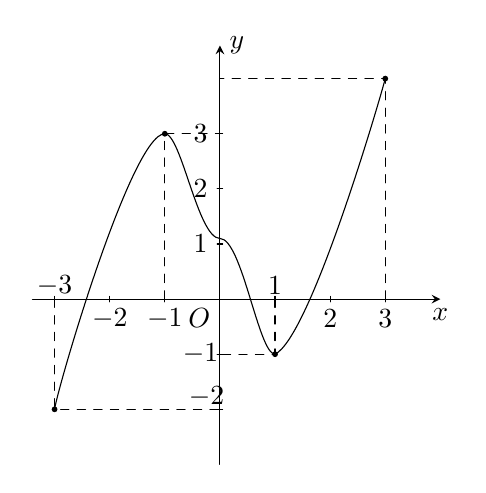
\begin{tikzpicture}[>=stealth,scale=.7, line join = round, line cap = round]
			\draw[->](-3.4,0)--(4,0)node[below]{$x$};
			\draw[->] (0,-3)--(0,4.6)node[right]{$y$};
			\draw (0,0)node[below left]{$O$};
			\draw (-3,-2)..controls+(82:.4)and+(180:.6)..(-1,3)..controls+(0:.3) and+(180:.4)..(0,1.1)..controls+(0:.4)and+(180:.3)..(1,-1)..controls+(26:.7)and+(-105:.6)..(3,4);
			\foreach \x/\g in {-3/90,-2/-90,-1/-90,1/90,2/-90,3/-90}\draw (\x,.05)--(\x,-.05)+(\g:.3)node{$\x$};
			\foreach \x/\g in {-2/130,-1/180,1/180,2/180,3/180}\draw (.05,\x)--(-.05,\x)+(\g:.3)node{$\x$};
			\draw[dashed] (-3,0)--(-3,-2)--(0,-2) (-1,0)--(-1,3)--(0,3) (3,0)--(3,4)--(0,4) (1,0)--(1,-1)--(0,-1);
			\fill[black] (-3,-2) circle(1.5pt);
			\fill[black] (-1,3) circle(1.5pt);
			\fill[black] (1,-1) circle(1.5pt);
			\fill[black] (3,4) circle(1.5pt);
		\end{tikzpicture}
	}
	\loigiai{
		Theo hình vẽ, hàm số đồng biến trên $(1;3)$.
	}
\end{ex}
%Câu 3 - Cực trị
\begin{ex}%[2D1N2-1]%[Dự án D - đợt 4 NH24-25- Hieu Hieu Minh Minh]
	Cho hàm số $y=\dfrac{2x^2-x-4}{x-1}$ có tất cả bao nhiêu điểm cực trị?
	\choice
	{$1$}
	{$2$}
	{\True $0$}
	{$3$}
	\loigiai{
		Tập xác định $\mathscr{D}=\mathbb{R}\setminus\{1\} $.\\
		$ y'=\dfrac{2x^2-4x+5}{(x-1)^2}=\dfrac{2(x-1)^2+3}{(x-1)^2}>0,\forall x\in \mathscr{D}$.\\
		Suy ra hàm số không có cực trị.
	}
\end{ex}
%Câu 4 - Cực trị
\begin{ex}%[2D1N2-2]%[Dự án D - đợt 4 NH24-25- Hieu Hieu Minh Minh]
	Cho hàm số $f(x)$ có bảng biến thiên như sau:
	\begin{center}
		
\begin{tikzpicture}
			\tkzTabInit[nocadre=false,lgt=1.2,espcl=2.5,deltacl=0.5]
			{$x$/0.6,$f'(x)$/0.6,$f(x)$/2}
			{$-\infty$,$-2$,$2$,$+\infty$}
			\tkzTabLine{,-,0,+,0,-,}
			\tkzTabVar{+/$+\infty$,-/$-1$,+/$3$,-/$-\infty$}
		\end{tikzpicture}
	\end{center}
	Giá trị cực tiểu của hàm số đã cho bằng
	\choice
	{$2$}
	{\True $-1$}
	{$-2$}
	{$3$}
	\loigiai{
		Dựa vào bảng biến thiên, giá trị cực tiểu của hàm số đã cho bằng $-1$.
	}
\end{ex}
%Câu 5 - GTNN
\begin{ex}%[2D1H3-1]%[Dự án D - đợt 4 NH24-25- Hieu Hieu Minh Minh]
	Giá trị nhỏ nhất của hàm số $y=\dfrac{-2x+3}{x+1}$ trên đoạn $[1;4]$ bằng bao nhiêu?
	\choice
	{$-\dfrac{9}{10}$}
	{$\dfrac{1}{2}$}
	{$1$}
	{\True $-1$}
	\loigiai{
		Ta có $y'=\dfrac{-5}{(x+1)^2}<0$, $\forall x\in [1;4]$ nên
		$\min\limits_{[1;4]} f(x)=f(4)=-1$.
	}
\end{ex}
%Câu 6 - GTNN
\begin{ex}%[2D1N3-1]%[Dự án D - đợt 4 NH24-25- Hieu Hieu Minh Minh]
	\immini[thm]{
		Cho hàm số $y=f(x)$ liên tục trên $\mathbb{R}$ và có đồ thị như hình vẽ. Gọi $M$ và $m$ lần lượt là giá trị lớn nhất và giá trị nhỏ nhất của hàm số $y=f(x)$ trên đoạn $[-1;3]$. Tìm $M$ và $m$.
		\choice
		{$M=3$; $m=0$}
		{$M=3$; $m=-1$}
		{$M=2$; $m=-4$}
		{\True $M=0$; $m=-4$}
	}
	{
		\begin{tikzpicture}[scale=.7,line cap=butt,line join=miter,>=stealth,font=\normalsize]
			\draw[->] (-2,0)--(4,0)	node[shift={(-100:7pt)}]{$x$};
			\draw[->] (0,-5)--(0,1)node[shift={(180:7pt)}]{$y$};
			\draw (5pt,0) |- (0,5pt) (0,0) node[shift={(225:9pt)}]{$O$};
			\tikzset{declare function={f(\x)=-(\x)^3+3*(\x)^2-4;}}
			\fill  (-1,0)node[below left]{$-1$}circle(1pt)
			(2,0)node[above]{$2$}circle(1pt)
			(1,0)node[above]{$1$}circle(1pt)
			(0,-4)node[below left]{$-4$}circle(1pt)
			(0,-2)node[left]{$-2$}circle(1pt)
			(3,0)node[above]{$3$}circle(1pt)
			(0,0)circle(1pt)
			;
			\draw[dashed] (0,-2)--(1,-2)--(1,0) (0,-4)--(3,-4)--(3,0)
			;
			\begin{scope}
				\clip (-5,-5) rectangle (5,1); 
				\draw[samples=100] plot[domain=-1.1:3.2] (\x, {f(\x)});
			\end{scope}
			\fill[black] (1,-2) circle(1.5pt);
			\fill[black] (3,-4) circle(1.5pt);
	\end{tikzpicture}
}
	\loigiai{Dựa vào đồ thị ta có $M=0$; $m=-4$.}
\end{ex}
%Câu 7 - Tiệm cận
\begin{ex}%[2D1H4-1]%[Dự án D - đợt 4 NH24-25- Hieu Hieu Minh Minh]
	Tiệm cận ngang của đồ thị hàm số $y=\dfrac{2x+3}{-x+4}$ là đường thẳng có phương trình
	\choice
	{$y=4$}
	{$x=-2$}
	{\True $y=-2$}
	{$x=4$}
	\loigiai{Ta có $\lim\limits_{x\rightarrow +\infty}\dfrac{2x+3}{-x+4}=\lim\limits_{x\rightarrow +\infty}\dfrac{2+\dfrac{3}{x}}{-1+\dfrac{4}{x}}=-2$.\\
		Tương tự, $\lim\limits_{x\rightarrow -\infty}\dfrac{2x+3}{-x+4}=-2$.\\
		Vậy đồ thị hàm số  $y=\dfrac{2x+3}{-x+4}$ có tiệm cận ngang là đường thẳng $y=-2$.}
\end{ex}
%Câu 8 - Tiệm cận
\begin{ex}%[2D1H4-3]%[Dự án D - đợt 4 NH24-25- Hieu Hieu Minh Minh]
	Cho hàm số $y=f(x)$ có đồ thị như hình vẽ đưới đây
	\begin{center}
		\begin{tikzpicture}[x=1cm,y=1cm,scale=0.7,>=stealth,declare function={a=1;b=2;c=-1;m=2;p=-2;},font=\footnotesize]
			\def\xmin{-5} \def\xmax{5}
			\def\ymin{-4} \def\ymax{5} 
			\def\f(#1){(a*(#1)^2+b*(#1)+c)/(m*(#1)^2+p)}
			\foreach \x in {-4,-3,-2,-1,1,2,3,4} \draw (\x,2pt)--(\x,-2pt) node [below] {$\x$};
			\draw[-stealth] (\xmin,0)--(\xmax,0)node[below]{$x$}; 
			\foreach \y in {-3,-2,-1,1,2,3,4} \draw (2pt,\y)--(-2pt,\y) node [left] {$\y$}; 
			\draw[-stealth] (0,\ymin)--(0,\ymax)node[right]{$y$}; 
			\filldraw (0,0)node[below left]{$O$} circle (1.5pt); 
			\clip (\xmin,\ymin) rectangle (\xmax,\ymax);  
			\draw[samples=100,domain=\xmin:p/m-0.1,smooth,red,thick] plot (\x,{\f(\x)});
			\draw[samples=100,domain=-p/m+0.1:\xmax,smooth,red,thick] plot (\x,{\f(\x)});
			\draw[samples=100,domain=p/m+0.1:-p/m-0.1,smooth,red,thick] plot (\x,{\f(\x)});
			\draw[samples=100,domain=\xmin:\xmax,smooth,dashed] plot (\x, {a/m}); 
			\draw[samples=100,domain=\ymin:\ymax,smooth,dashed] plot ({-p/m},\x);
			\draw[samples=100,domain=\ymin:\ymax,smooth,dashed] plot ({p/m},\x);
			\draw[samples=100,domain=\ymin:\ymax,smooth,dashed] plot ({1},\x);
			\filldraw (0,0.5)node[above right]{$\tfrac{1}{2}$} circle (1.5pt);	
		\end{tikzpicture}	
	\end{center}
	Tổng số tiệm cận đứng và tiệm cận ngang của đồ thị hàm số $y=f(x)$ là
	\choice
	{$2$}
	{$4$}
	{\True $3$}
	{$6$}
	\loigiai{
		Ta có $\heva{& \lim\limits_{x \to -1^\pm} f(x)=\pm\infty \\ & \lim\limits_{x \to 1^\pm} f(x)=\mp\infty}\Rightarrow\heva{& x=-1 \\ & x=1}$ là hai đường tiệm cận đứng của đồ thị hàm số.\\
		$\lim\limits_{x \to \pm\infty} f(x)=\dfrac{1}{2}\Rightarrow y=\dfrac{1}{2}$ là đường tiệm cận ngang của đồ thị hàm số. \\
		Vậy đồ thị hàm số có $3$ đường tiệm cận.
	}
\end{ex}
%Câu 9 - Tiệm cận
\begin{ex}%[2D1N4-1]%[Dự án D - đợt 4 NH24-25- Hieu Hieu Minh Minh]
	Cho hàm số $y=f(x)=-x-6+\dfrac{1}{x+1}$. Tìm tiệm cận xiên của đồ thị hàm số đã cho. 
	\choice
	{\True $y=-x-6$}
	{$y=-x$}
	{$x=-1$}
	{$y=0$}
	\loigiai{
		Ta có
		$\lim\limits_{x\to+\infty}[f(x)-(-x-6)]=\lim\limits_{x\to+\infty}\dfrac{1}{x+1}=0$.\\
		Vậy tiệm cận xiên của đồ thị hàm số là $y=-x-6$.
	}
\end{ex}
%Câu 10 - Đồ thị
\begin{ex}%[2D1H5-1]%[Dự án D - đợt 4 NH24-25- Hieu Hieu Minh Minh]
	\immini[thm]{Đồ thị hàm số nào dưới đây có dạng đường cong như hình vẽ?
		\choice
		{$y=-x^3+3x+1$}
		{$y=\dfrac{x-1}{x+2}$}
		{\True $y=x^3-3x+1$}
		{$y=\dfrac{x^2+3}{x+2}$}}
	{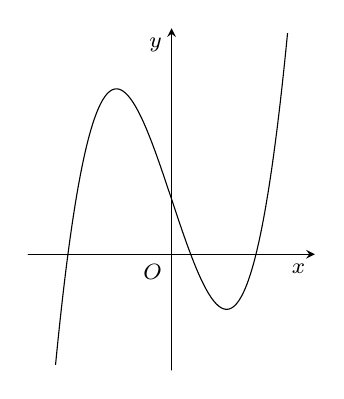
\begin{tikzpicture}[scale=0.7, font=\footnotesize, line join=round, line cap=round,>=stealth]
			\tikzset{every node/.style={scale=1}}
			\draw[->] (-2.6,0)--(2.6,0) node[below left] {$x$};
			\draw[->] (0,-2.1)--(0,4.1) node[below left] {$y$};
			\draw (0,0) node [below left] {$O$};
			\begin{scope}
				\clip (-2.5,-2) rectangle (2.5,4);
				\draw[samples=200,domain=-2.5:2.5,smooth,variable=\x] plot (\x,{1*((\x)^3)-3*(\x)+1});
			\end{scope}
	\end{tikzpicture}}
	\loigiai{
		Từ đồ thị suy ra hàm số có dạng $y=ax^3+bx^2+cx+d$, có $a>0$ và $d>0$.\\
		Trong các hàm số đã cho chỉ có hàm số $y=x^3-3x+1$ thỏa mãn.
	}
\end{ex}
%Câu 11 - Đồ thị
\begin{ex}%[2D1N5-1]%[Dự án D - đợt 4 NH24-25- Hieu Hieu Minh Minh]
	\immini[thm]{
		Đồ thị của hàm số nào dưới đây có dạng đường cong như hình vẽ?
		\choice
		{$y=\dfrac{x+1}{x-1}$}
		{$y=\dfrac{x}{x+2}$}
		{$y=\dfrac{x}{x+1}$}
		{\True $y=\dfrac{x}{x-1}$}
	}
	{
		\begin{tikzpicture}[scale=0.7,line join=round, line cap=round,>=stealth]
			\tikzset{every node/.style={scale=1}}
			\draw[->] (-3.1,0)--(4.1,0) node[below left] {$x$};
			\draw[->] (0,-2.1)--(0,4.1) node[below left] {$y$};
			\draw (0,0) node [below left] {$O$};
			\draw[thin] (1,1pt)--(1,-1pt) node [below left] {$1$};
			\draw[dashed,thin] (1.01,-2)--(1.01,4);
			\begin{scope}
				\clip (-3,-2) rectangle (4,4);
				\draw[samples=200,domain=-3:0.99,smooth,variable=\x] plot (\x,{(1*(\x)+0)/(1*(\x)+-1)});
				\draw[samples=200,domain=1.01:4,smooth,variable=\x] plot (\x,{(1*(\x)+0)/(1*(\x)+-1)});
				\draw[dashed,thin] (-3,1/1)--(4,1/1);
			\end{scope}
		\end{tikzpicture}
	}
	\loigiai{
		Đồ thị có tiệm cận đứng là $x=1$ và đi qua $O(0;0)$ nên đồ thị đã cho là của hàm số $y=\dfrac{x}{x-1}$.
	}
\end{ex}
%Câu 12 - Đồ thị
\begin{ex}%[2D1H5-1]%[Dự án D - đợt 4 NH24-25- Hieu Hieu Minh Minh]
	\immini{
		Đồ thị trong hình bên là đồ thị của hàm số
		\choice
		{$y=\dfrac{x^2-x+1}{x+1}$}
		{\True $y=\dfrac{x^2+x+1}{x+1}$}
		{$y=x-\dfrac{1}{x+1}$}
		{$y=\dfrac{2x+1}{x+1}$}	
	}
	{
		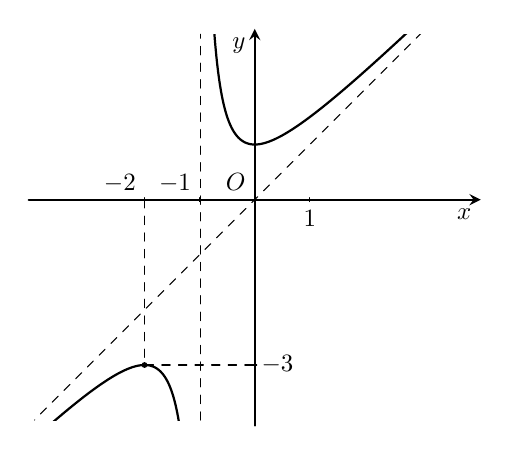
\begin{tikzpicture}[line join=round, line cap=round,>=stealth,thick,scale=.7]
			\tikzset{every node/.style={scale=0.9}}
			\draw[->] (-4.1,0)--(4.1,0) node[below left] {$x$};
			\draw[->] (0,-4.1)--(0,3.1) node[below left] {$y$};
			\draw (0,0) node [above left] {$O$};
			\foreach \x/\nx in {1/1}
			\draw[thin] (\x,1pt)--(\x,-1pt) node [below] {$\nx$};
			\foreach \x/\nx in {-2/-2,-1/-1}
			\draw[thin] (\x,1pt)--(\x,-1pt) node [above left] {$\nx$};
			\foreach \y/\ny in {-3/-3}
			\draw[thin] (1pt,\y)--(-1pt,\y) node [right] {$\ny$};
			\draw[dashed,thin](-2,0)--(-2,-3)--(0,-3);
			\draw[dashed,thin] (-0.99,-4)--(-0.99,3);
			\begin{scope}
				\clip (-4,-4) rectangle (4,3);
				\draw[samples=200,domain=-4:-1.01,smooth,variable=\x] plot (\x,{(1*((\x)^2)+1*(\x)+1)/(1*(\x)+1)});
				\draw[samples=200,domain=-0.99:5,smooth,variable=\x] plot (\x,{(1*((\x)^2)+1*(\x)+1)/(1*(\x)+1)});
				\draw[dashed,thin] (-4.1,-4.1)--(5.1,5.1);
			\end{scope}
			\fill[black](-2,-3) circle(1.5pt);
		\end{tikzpicture}	
	}
	\loigiai{
		Từ hình vẽ ta thấy
		\begin{itemize}
			\item Đây là đồ thị của hàm số có dạng $y=\dfrac{ax^2+bx+c}{mx+n}$ với $m\neq 0$ nên loại hàm số $y=\dfrac{2x+1}{x+1}$.
			\item Đồ thị hàm số đi qua điểm $(-2;-3)$ nên loại hàm số $y=\dfrac{x^2-x+1}{x+1}$ và $y=x-\dfrac{1}{x+1}$.
		\end{itemize}
		Vậy đồ thị trong hình vẽ là đồ thị của hàm số $y=\dfrac{x^2+x+1}{x+1}$.
	}
\end{ex}
\Closesolutionfile{ans}
%\begin{center}
%	\textbf{ĐÁP ÁN}
%	\inputansbox{10}{ans/ans}	
%\end{center}

\begin{center}
	\textbf{PHẦN 2 - CÂU TRẮC NGHIỆM ĐÚNG SAI}
\end{center}
\setcounter{ex}{0}
\Opensolutionfile{ans}[ans/answer-DS-ONTAPCHUONG1-DE3]

%Câu 1%
\begin{ex}%[2D1H4-1]%[Dự án D - đợt 4 NH24-25- Hieu Hieu Minh Minh]
	Cho hàm số $f(x)=\dfrac{3x^2+5x-4}{6x-2}$ có đồ thị $(C)$. 
	\choiceTF
	{\True Hàm số có tập xác định là $\mathbb{R}\setminus \left\{\dfrac{1}{3}\right\}$}
	{\True Đạo hàm $f'(x)=\dfrac{9x^2-6x+7}{2(3x-1)^2}$}
	{\True Hàm số không có cực trị}
	{Hàm số luôn luôn nghịch biến trên từng khoảng xác định}
	\loigiai{
		\begin{itemchoice}
			\itemch Điều kiện xác định $6x-2\neq 0\Leftrightarrow x\neq \dfrac{1}{3}$.\\
			Tập xác định $\mathscr{D}=\mathbb{R}\setminus \left\{\dfrac{1}{3}\right\}$.
			\itemch Ta có \begin{eqnarray*}
				f'(x)&=&\dfrac{(3x^2+5x-4)'\cdot(6x-2)-(3x^2+5x-4)\cdot (6x-2)'}{(6x-2)^2}\\
				&=&\dfrac{(6x+5)\cdot(6x-2)-6(3x^2+5x-4)}{4(3x-1)^2}\\
				&=& \dfrac{36x^2+18x-10-18x^2-30x+24}{4(3x-1)^2}\\
				&=& \dfrac{18x^2-12x+14}{4(3x-1)^2}\\
				&=& \dfrac{9x^2-6x+7}{2(3x-1)^2}.
			\end{eqnarray*}
			\itemch Cho $y'=0\Leftrightarrow 9x^2-6x+7=0$ 
			(vô nghiệm vì $9x^2-6x+7=(3x-1)^2+6>0$, $\forall x$).\\
			Vậy hàm số không có cực trị.
			\itemch Vì $f'(x)>0, \forall x \in \mathbb{R}$ nên hàm số luôn luôn đồng biến trên từng khoảng xác định.
		\end{itemchoice}
	}
\end{ex}
%Câu 2%
\begin{ex}%[2D1H5-1]%[Dự án D - đợt 4 NH24-25- Hieu Hieu Minh Minh]
	\immini{
		Cho hàm số $y=\dfrac{x+a}{bx+c}$ với $a$, $b$, $c\in \mathbb{Z}$ và $b\ne 0$ có đồ thị như hình vẽ bên.
		\choiceTF
		{Hàm số đồng biến trên $(-\infty;1)\cup (1;+\infty)$}
		{Đồ thị hàm số có tiệm cận ngang $y=0$}
		{\True $T=a-3b-2c=-3$}
		{\True Đồ thị hàm số có tiệm cận đứng $x=1$}
	}{
		\begin{tikzpicture}[scale=0.6,line join=round, line cap=round,>=stealth]
			\def\xmin{-4} \def\xmax{5}
			\def\ymin{-3} \def\ymax{5}
			\draw[->] (\xmin,0)--(\xmax,0) node[below] {$x$};
			\draw[->] (0,\ymin)--(0,\ymax) node[left] {$y$};
			\draw (0,0) node [below left] {$O$};
			\foreach \x/\g in {1/-145,2/-35}
			\draw[thin] (\x,1pt)--(\x,-1pt)+(\g:0.4)node[scale=1]{$\x$};
			\foreach \y/\g in {1/145,2/145}		
			\draw[thin] (1pt,\y)--(-1pt,\y)+(\g:0.4)node[scale=1]{$\y$};
			\begin{scope}
				\clip (\xmin+0.1,\ymin+0.1) rectangle (\xmax-0.1,\ymax-0.1);
				\draw[red,smooth,samples=300,domain=1.01:\xmax] plot(\x,{(1*(\x)-2)/(\x-1)});
				\draw[red,smooth,samples=300,domain=\xmin:0.99] plot(\x,{(1*(\x)-2)/(\x-1)});
				\draw[dashed,blue,smooth,samples=300,domain=\xmin:\xmax] plot(\x,{1});
				\draw[dashed,blue] (1,\ymin)--(1,\ymax);
			\end{scope}
			\foreach \x/\y in {0/1,1/0,2/0,0/2}
			\fill[black] (\x,\y) circle(1.2pt);
		\end{tikzpicture}
	}	
	\loigiai{
		Theo đồ thị, ta có tiệm cận ngang $y=1=\dfrac{1}{b}\Rightarrow b=1$.\\
		Tiệm cận đứng $x=1=\dfrac{-c}{b}=\dfrac{-c}{1}\Rightarrow c=-1$.\\
		Đồ thị hàm số cắt trục tung tại $(0;2)$ nên ta có $\dfrac{0+a}{1\cdot 0-1}=2\Rightarrow a=-2$.
		\begin{itemchoice}
			\itemch Hàm số đồng biến trên từng khoảng $(-\infty;1)$, $(1;+\infty)$.
			\itemch Vì hàm số có tiệm cận ngang $y=1$.
			\itemch Ta có $T=a-3b-2c=-2-3+2=-3$.
			\itemch Vì hàm số có tiệm cận đứng $x=1$.
		\end{itemchoice}
	}
\end{ex}
\Closesolutionfile{ans}
%\inputansbox[2]{2}{ans/answer.tex}
%
\begin{center}
\textbf{PHẦN 3 - CÂU TRẮC NGHIỆM TRẢ LỜI NGẮN}
\end{center}
\setcounter{ex}{0}
\Opensolutionfile{ans}[ans/ans-KQ-ONTAPCHUONG1-DE3]
%Câu 1%
\begin{ex}%[2D1H2-1]%[Dự án D - đợt 4 NH24-25- Hieu Hieu Minh Minh]
	Đồ thị hàm số $y=x^3-3 x^2+m$ có điểm cực tiểu là $M(a ; b)$ và $a+b=1$. Tìm giá trị $m$.
	\shortans{3}
	\loigiai{
		Ta có $y'=3x^2-6x$.\\
		Cho $y'=0\Leftrightarrow \hoac{&x=0\\&x=2.}$\\
		Bảng biến thiên
		\begin{center}
			
\begin{tikzpicture}
				\tkzTabInit[nocadre=false,lgt=1,espcl=2,deltacl=0.5]
				{$x$/.6 ,$y'$/.6,$y$/2}
				{$-\infty$ , $0$ , $2$ , $+\infty$}
				\tkzTabLine{ , + , $0$ , - , $0$ , + , }
				\tkzTabVar{-/$-\infty$ , +/$m$ , -/$m-4$ , +/$+\infty$}
			\end{tikzpicture}
		\end{center}
		Đồ thị hàm số có điểm cực tiểu là $(2;m-4)$, theo giả thiết đồ thị hàm số có điểm cực tiểu là $M(a ; b)$ và $a+b=1$.\\
		Suy ra $2+ m-4=1\Leftrightarrow m=3$.
	}
\end{ex}
%Câu 2%
\begin{ex}%[2D1V3-6]%[Dự án D - đợt 4 NH24-25- Hieu Hieu Minh Minh]
	Ông A dự định đầu tư sản xuất một loại sản phẩm với số lượng không quá $200$ sản phẩm. Nếu ông A bán được $x$ sản phẩm thì thu về số tiền tính theo công thức $f(x)=x^3-1550 x^2+128500 x+30000$ (đồng). Chi phí sản xuất bình quân cho một sản phẩm được tính theo công thức $C(x)=1000+x+\dfrac{25000}{x}$ (đồng). Ông A cần sản xuất bao nhiêu sản phẩm thì lợi nhuận thu về là lớn nhất, (sản phẩm là một số nguyên)?
	\shortans{43}
	\loigiai{
		Lợi nhuận $L(x)$ được xác định bằng
		$$
		L(x)=f(x)-C(x) \cdot x.
		$$	
		Trong đó
		\begin{itemize}
			\item $f(x)=x^3-1550 x^2+128500 x+30000$ là tổng doanh thu khi bán $x$ sản phẩm.
			\item $C(x)$ là chi phí bình quân cho một sản phẩm, vậy tổng chi phí là $C(x) \cdot x$
		\end{itemize}
		$$
		C(x) \cdot x=\left(1000+x+\frac{25000}{x}\right) \cdot x=1000 x+x^2+25000.
		$$
		Thay vào, ta có
		\begin{eqnarray*}
			L(x)&=&\left(x^3-1550 x^2+128500 x+30000\right)-\left(1000 x+x^2+25000\right) 
			\\&=&x^3-1551 x^2+127500 x+5000.
		\end{eqnarray*}
		Ta có $L'(x)=3 x^2-3102 x+127500$, cho $L'(x)=0\Leftrightarrow \hoac{&x\approx 42{,}9 \,\text{ (nhận)}\\& x\approx 991{,}1\,\text{ (loại)}.}$\\
		Bảng biến thiên
		\begin{center}
			
\begin{tikzpicture}
				\tkzTabInit[nocadre=false,lgt=1.5,espcl=2,deltacl=0.5]
				{$x$/.6 ,$L'(x)$/.6,$L(x)$/2}
				{$0$ , $42{,}9$ , $200$}
				\tkzTabLine{ , + , $0$ , - , }
				\tkzTabVar{-/$ $ , +/$ $ , -/$ $}
			\end{tikzpicture}
		\end{center}
		Do sản phẩm là một số nguyên nên xét $L(42)=2\,698\,124$ và $L(43)=2\,699\,208$.\\
		Vậy sản xuất $43$ sản phẩm là lợi nhuận đạt tối đa.
	}
\end{ex}
%Câu 3%
\begin{ex}%[2H2H2-6]%[Dự án D - đợt 4 NH24-25- Hieu Hieu Minh Minh]
	Nhà máy A chuyên sản xuất một loại sản phẩm cung cấp cho nhà máy B. Hai nhà máy thoả thuận rằng, hằng tháng A cung cấp cho B số lượng sản phẫm theo đơn đặt hàng của B (tối đa 100 tấn sản phẩm). Nếu số lượng đặt hàng là $x$ tấn sản phẩm thì giá bán cho mỗi tấn sản phẩm là $\mathrm{P}(x)=45-0,001x^2$ (triệu đồng). Chi phí để A sản xuất $x$ tấn sản phẩm trong một tháng là $\mathrm{C}(x)=100+30x$ (triệu đồng) (gồm $100$ triệu đồng chi phí cố định và $30$ triệu đồng cho mỗi tấn sản phẩm). Lợi nhuận lớn nhất mà nhà máy A thu được mỗi tháng là $a$ triệu đồng. Tìm $a$ (làm tròn đến hàng đơn vị).
	\shortans{707}
	\loigiai{
		Doanh thu của nhà máy khi sản xuất 1 tấn sản phẩm là $P(x)$ triệu đồng.\\
		Doanh thu của nhà máy khi sản xuất $x$ tấn sản phẩm là $x P(x)$ triệu đồng.\\
		Chi phí của nhà máy khi sản xuất $x$ tấn sản phẩm là $C(x)$ triệu đồng.\\
		Ta có lợi nhuận của nhà máy A khi sản xuất $x$ tấn sản phẩm là \allowdisplaybreaks
		\begin{eqnarray*}
			H(x)&=&x P(x)-C(x)\\
			&=&x\left(45-0,001 x^2\right)-(100+30 x)\\
			&=& -0{,}001 x^3+15x-100, \text { với } 0 \leqslant x \leqslant 100.
		\end{eqnarray*}
		$H^{\prime}(x)=-0{,}003 x^2+15$.\\
		$H^{\prime}(x)=0\Leftrightarrow -0{,}003x^2+15=0\Leftrightarrow\hoac{&x=50\sqrt{2} \\ &x=-50\sqrt{2}.}$\\
		Chỉ có $x=50 \sqrt{2}$ thỏa mãn điều kiện.\\
		Ta có: $H(0)=-100$; $H(50 \sqrt{2})=500 \sqrt{2}\approx 707$; $H(100)=400$.\\
		Vậy lợi nhuận lớn nhất của nhà máy $A$ là $707$ triệu đồng.
	}
\end{ex}
%Câu 4%
\begin{ex}%[2D1V4-2]%[Dự án D - đợt 4 NH24-25- Hieu Hieu Minh Minh]
	Cho hàm số $ y=\dfrac{x+3}{x^2-6x+m} $, với $m$ là tham số thực. Số các giá trị của tham số $m$ để đồ thị của hàm số chỉ có một tiệm cận đứng và một tiệm cận ngang. 
	\shortans{2}
	\loigiai{
		Ta có $ \lim\limits_{x\to +\infty}y=\lim\limits_{x\to -\infty}y=0 $ nên đồ thị hàm số có $ 1 $ đường tiệm cận ngang là $y=0$.\\	
		Đồ thị hàm số đã cho cần có $1$ tiệm cận đứng khi phương trình $x^2-6x+m=0$ có nghiệm kép hoặc có $2$ nghiệm phân biệt trong đó có một nghiệm bằng $-3$.\\ Điều kiện tương đương là \[\hoac{& \Delta'=(-3)^2-1\cdot m=0 \\ & \heva{&\Delta'=(-3)^2-1\cdot m>0\\ & (-3)^2-6\cdot (-3)+m=0}}\Leftrightarrow\hoac{& m=9 \\ & \heva{& m<9 \\ & m=-27}}\Leftrightarrow\hoac{& m=9 \\ & m=-27.}\]
		Vậy các giá trị $m$ cần tìm là $m=9$, $m=-27$.	
	}
\end{ex}
\Closesolutionfile{ans}
\begin{center}
	\textbf{PHẦN 4 - TỰ LUẬN}
\end{center}
\setcounter{ex}{0}
%Câu 1%
\begin{ex}%[2D1H5-7]%[Dự án D - đợt 4 NH24-25- Hieu Hieu Minh Minh]
	Cho hàm số $y=x^3-3x^2+5$ có đồ thị $(C)$, gọi $A(x;y)$ là điểm cực đại của đồ thị hàm số. Tính $x+2y$.
	\loigiai
	{
		Ta có $y'=3x^2-6x$. \\
		Xét $y'=0 \Leftrightarrow \hoac{ & x=0 \\ & x=2.}$ \\
		Bảng biến thiên
		\begin{center}
			
\begin{tikzpicture}
				\tkzTabInit[nocadre=false, lgt=1.2, espcl=2.5, deltacl=0.6]{$x$/0.6, $y'$/0.6, $y$/2}{$-\infty$, $0$, $2$, $+\infty$}
				\tkzTabLine{,+,0,-,0,+,}
				\tkzTabVar{-/$-\infty$, +/$5$, -/$1$, +/$+\infty$}
			\end{tikzpicture}
		\end{center}
		Từ bảng biến thiên, ta có $A(0;5)$ là điểm cực đại của đồ thị hàm số.\\
		Suy ra $x=0$; $y = 5$.\\
		Vậy $x+2y=0+2\cdot5=10$.
	}
\end{ex}
%Câu 2%
\begin{ex}%[2D1V3-1]%[Dự án D - đợt 4 NH24-25- Hieu Hieu Minh Minh]
	Cho hàm số $y=\sqrt{4x-2x^2}$. Gọi $M$ là giá trị lớn nhất và $m$ là giá trị nhỏ nhất của hàm số. Tính giá trị $M^{26}+m^{2\,026}$.
	\loigiai{
		Tập xác định của hàm số là $\mathscr{D} = [0;2]$, ta tìm giá trị nhỏ nhất và giá trị lớn nhất của hàm số trên $\mathscr{D}$.
		\begin{itemize}
			\item $y=\sqrt{4x-2x^2} \Rightarrow y'=\dfrac{(4x-2x^2)'}{2\sqrt{4x-2x^2}}=\dfrac{-2x+2}{\sqrt{4x-2x^2}}$.
			\item $y'=0 \Rightarrow x = 1 \in \mathscr{D}$.
		\end{itemize}
		Ta tính được $y(0)=0$, $y(1)=\sqrt{2}$, $y(2)=0$.\\
		Vậy $M=\sqrt{2}$, $m=0$.\\
		Khi đó $M^{26}+m^{2\,026}={\sqrt{2}}^{26}+0^{2\,026}=8\,192$.
	}
\end{ex}
%Câu 3%
\begin{ex}%[2D1V5-1]%[Dự án D - đợt 4 NH24-25- Hieu Hieu Minh Minh]
	Cho hàm số bậc ba $y=f(x)$ có đồ thị như hình vẽ bên dưới.
	\begin{center}
		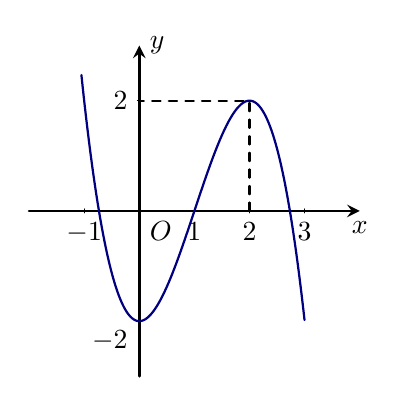
\begin{tikzpicture}[scale=0.7, line join = round, line cap = round,>=stealth,thick,x = 1cm,y = 1cm] 
		%Vẽ hệ trục Oxy 
		\draw[->,line width = 1pt] (-2,0)--(0,0) node[below right]{$O$}--(4,0) node[below]{$x$}; 
		\draw[->,line width = 1pt] (0,-3)--(0,3) node[right]{$y$}; 
		%Vẽ các điểm trên hệ trục 
		\foreach \x in {-1,1,2,3} \draw[thin] (\x,1pt)--(\x,-1pt) node [below] {$\x$}; 
		\foreach \y in {-2} \draw[thin] (1pt,\y)--(-1pt,\y) node [below left] {$\y$};
		\foreach \y in {2} \draw[thin] (1pt,\y)--(-1pt,\y) node [ left] {$\y$};  
		%Vẽ đồ thị hàm số 
		\draw[dashed] (2,0)--((2,2)--(0,2);
		\draw[samples=200,domain=-1.05:3.0,smooth,blue!50!black] plot (\x, {-(\x)^3+3*(\x)^2-2}) node[right,red]{$ $}; 
		\end{tikzpicture}
	\end{center}
	Tính giá trị của $f(-2)$.
	\loigiai{
		Hàm số bậc ba cần tìm có dạng $y=f(x)=ax^3+bx^2+cx+d$ với $a\ne 0$.\\
		Suy ra $f'(x)=3ax^2+2bx+c$.\\
		Từ bảng biến thiên, ta có
		$\heva{&f(0)=-2\\&f(2)=2\\&f'(0)=0\\&f'(2)=0} \Leftrightarrow \heva{&d=-2\\&8a+4b+2c+d=2\\&c=0\\&12a+4b+c=0.}$\\
		Giải hệ trên ta được $ a=-1,b=3,c=0,d=-2$.\\
		Vậy $f(x)=-x^3+3x^2-2 \Rightarrow f(-2)=-(-2)^3+3\cdot(-2)^2-2=18$.
	}
\end{ex}